%
% Wissenschaftliches Arbeiten mit LaTeX
%
% @author Muhammad Juan Akbar
% @version 1.0
% 

\documentclass[a4paper,12pt]{scrreprt}
\usepackage{main_conf}

% ============= Dokumentbeginn =============
\begin{document}
%Seiten ohne Kopf- und Fußzeile sowie Seitenzahl
\pagestyle{empty}

\begin{center}
\begin{tabular}{p{\textwidth}}


\begin{center}

\includegraphics[scale=0.5]{img/htw-logo.png}
\end{center}


\\

\begin{center}
\LARGE{\textsc{
Bedeutung Über eine wichtige Sache\\
}}
\end{center}

\\
\\


\begin{center}
\large{AWE Wissenschaftliches Arbeiten mit LaTeX} \\
\end{center}

\\

\begin{center}
\textbf{\Large{Belegarbeiten}} \\
\end{center}


\\
\\


\begin{center}
vorgelegt von
\end{center}

\begin{center}
\large{\textbf{Muhammad Juan Akbar}} \\
\small{s0529263@htw-berlin.de}
\end{center}

\begin{center}
\large{s0529263} \\
\end{center}

\begin{center}
\begin{tabular}{lll}
\textbf{Erstprüfer:} & & Frau S. Kröger
\end{tabular}
\end{center}

\end{tabular}
\end{center}

% Beendet eine Seite und erzwingt auf den nachfolgenden Seiten die Ausgabe aller Gleitobjekte (z.B. Abbildungen), die bislang definiert, aber noch nicht ausgegeben wurden. Dieser Befehl fügt, falls nötig, eine leere Seite ein, sodaß die nächste Seite nach den Gleitobjekten eine ungerade Seitennummer hat. 
\cleardoubleoddpage

% pagestyle für gesamtes Dokument aktivieren
\pagestyle{fancy}

%Inhaltsverzeichnis
\tableofcontents

%Verzeichnis aller Bilder
\listoffigures

%Verzeichnis aller Tabellen
\listoftables

%----------------------------------------------------------------
% Chapter 1
% https://www.saxoprint.de/blog/unterschied-pixelgrafik-vektorgrafik/
%----------------------------------------------------------------
\chapter{Der Unterschied zwischen Pixel- und Vektorgrafiken}
\label{cha:der_unterschied_zwischen_pixel-_und_vektorgrafiken}
Druckprodukte in unterschiedlichster Art und Auflage werden längst nicht mehr nur von Unternehmen benötigt. Auch bei Privatpersonen ist der Bedarf inzwischen gestiegen. Um diesen zu decken, gibt es Druckereien wie wir, die die Möglichkeit bieten online Drucksachen wie Flyer, Visitenkarten, Briefbögen uvm. zu bestellen. Dies ist in den meisten Fällen kostengünstig und einfach händelbar. Das Aufbereiten und Übersenden von Druckdaten an die Druckerei setzt jedoch einige Grundkenntnisse in der Grafikbearbeitung voraus. Leider sind dem Laien jedoch diverse Fachbegriffe kaum geläufig, dass hin und wieder zu Missverständnissen führt und die Druckprodukte letztendlich nicht die gewünschte Qualität aufweisen. Daher zeige ich in diesem Blogartikel welche Unterschiede zwischen Vektor- und Pixelgrafiken existieren (siehe Abb \ref{fig:pixel_vector_exp}).

% images pixel & vector
\begin{figure}
\centering
	\begin{subfigure}[b]{5cm}            
		\frame{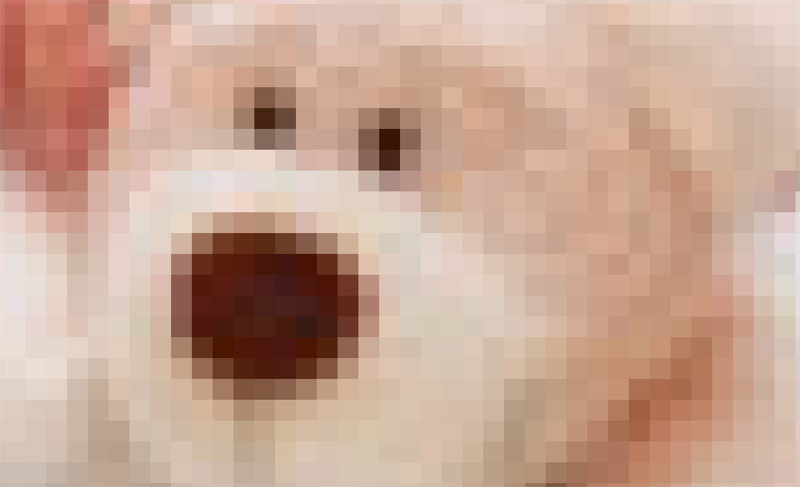
\includegraphics[width=5cm]{img/kapitel_1_pixel.jpg}}
		\caption{Pixelgrafik stark vergrößert}
		\label{fig:pixel}
	\end{subfigure}
%
\hspace{1cm}
%
	\begin{subfigure}[b]{5cm}
	\centering
		\frame{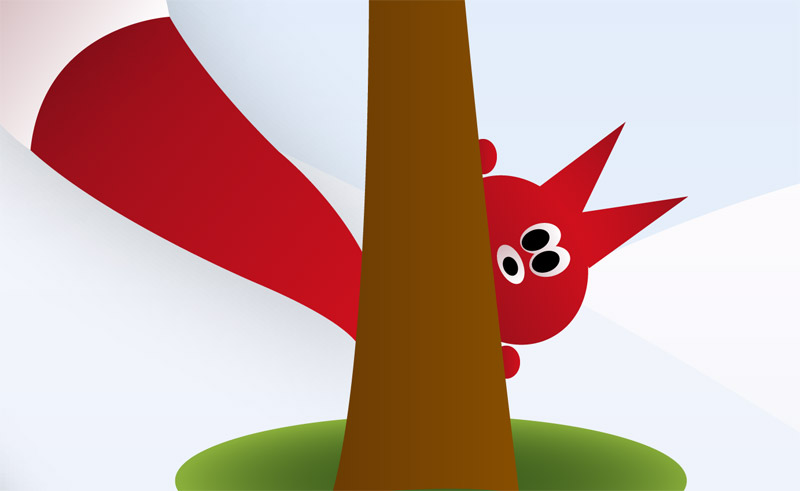
\includegraphics[width=5cm]{img/kapitel_1_vektor.jpg}}
		\caption{Vektorgrafik stark vergrößert}
		\label{fig:vector}
	\end{subfigure}

	\caption{Pixel- und Vektorgrafiken}
	\label{fig:pixel_vector_exp}
\end{figure}

%----------------------------------------------------------------
% Section 1
%----------------------------------------------------------------
\section{Vektorgrafiken – die Bildraster}
\label{sec:vektorgrafiken_-_die_bildraster}

Vektorgrafiken sind seltener im Internet zu finden, da sie im Consumer-Bereich nur wenig Anwendung finden. Sie bestehen nicht aus einzelnen kleinen Bildpunkten sondern sind aus geometrisch definierten Grundelementen zusammengesetzt und daher eher als mathematische Formelsammlung zu verstehen statt als Bildraster. So bestehen die einzelnen Vektoren aus Linien, Kurven, Kreisen oder Polygonen die in ihrer Zusammensetzung komplexe Grafiken ergeben können. Diese sogenannten Primitiven benötigen nur wenige Angaben. Bei einem Kreis ist dies zum Beispiel die Position des Kreismittelpunktes und sein Radius. Zudem lassen sich verschiedene Eigenschaften wie die Linienstärke, die Konturfarbe oder diverse Füllmuster und Verläufe festlegen.

Daher eigenen sich Vektorgrafiken besonders zur Darstellung von geometrischen Designs und Schriften. Zudem benötigen sie oft bedeutend weniger Speicherplatz als Pixelgrafiken und lassen sich verlustfrei vergrößern oder verkleinern, weshalb sie in der Druckindustrie einen hohen Stellenwert besitzen.

%----------------------------------------------------------------
% Section 2
%----------------------------------------------------------------
\section{Pixelgrafiken – die Rastergrafiken}
\label{sec:pixelgrafiken_-_die_rastergrafiken}

\begin{wrapfigure}{R}{0.3\textwidth}
\centering
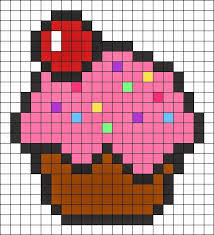
\includegraphics[width=0.15\textwidth]{img/k1_pixel_img.jpg}
\caption{\label{fig:frog1}Pixelgrafiken}
\end{wrapfigure}

Eine Pixelgrafik, auch Bitmap- oder Rastergrafik genannt, besteht hingegen aus einzelnen Bildpunkten, die in einem Raster angeordnet sind und denen jeweils ein Farbwert zugeordnet ist. Diese Grafikart definiert sich daher durch ihre Abmessung aus Höhe und Breite in Pixeln, die auch Bildauflösung genannt wird, sowie durch den Umfang der darstellbaren Farben, den man auch als Farbtiefe bezeichnet.

Rastergrafiken eigenen sich daher hervorragend zur Darstellung von Fotos und komplexen Farbverläufen. Ein großer Nachteil besteht jedoch in der starken Verschlechterung der Bildqualität sobald man diese Grafiken vergrößert, da durch die Rasterung ein sogenannter Treppeneffekt entsteht, welcher die Bilder dann pixelig oder unscharf wirken lässt. Zudem wird bei Bildformaten, wie zum Beispiel den JPG-Dateien, eine verlustbehaftete Bildkompression eingesetzt, welche die Qualität weiter mindern kann.
%----------------------------------------------------------------
% Chapter 2
% https://de.wikipedia.org/wiki/Matrix_(Mathematik)
%----------------------------------------------------------------
\chapter{Wichtige Mathematik Formeln}
\label{cha:wichtige_mathematik_formeln}


%----------------------------------------------------------------
% Section 1
%----------------------------------------------------------------
\section{Matrix}
\label{sec:matrix}
In der Mathematik versteht man unter einer Matrix (Plural Matrizen) eine rechteckige Anordnung (Tabelle) von Elementen (meist mathematischer Objekte, etwa Zahlen). Mit diesen Objekten lässt sich dann in bestimmter Weise rechnen, indem man Matrizen addiert oder miteinander multipliziert. Matrizen können beliebige Dimensionalität besitzen bspw. \ref{eq:matrix1}.
\vspace{5mm}
Matrizen sind ein Schlüsselkonzept der linearen Algebra und tauchen in fast allen Gebieten der Mathematik auf. Sie stellen Zusammenhänge, in denen Linearkombinationen eine Rolle spielen, übersichtlich dar und erleichtern damit Rechen- und Gedankenvorgänge.
\vspace{5mm}

\[ \begin{array}{|cccc|} \label{eq:matrix1}
a_{11} & a_{12} & \cdots & a_{1n} \\
a_{21} & a_{22} & \cdots & a_{21} \\
\vdots & \vdots & \ddots & \vdots \\
a_{m1} & a_{m2} & \cdots & a_{mn}
\end{array} \]

\begin{displaymath}
\left\{\begin{array}{cccc}
\Gamma_{11} & \Gamma_{12} & \cdots &
\Gamma_{1n}\\
\Gamma_{21} & \Gamma_{22} & \cdots &
\Gamma_{2n}\\
\vdots & \vdots & \ddots &
\vdots\\
\Gamma_{m1} & \Gamma_{m2} & \cdots &
\Gamma_{mn}
\end{array}\right\}
\end{displaymath}


%----------------------------------------------------------------
% Section 2
%----------------------------------------------------------------
\section{Ableitung}
\label{sec:ableitung}

Wie leitet man eine Funktion ab, die von "x" abhängt? In der Mathematik gibt es verschiedene Regeln um eine Funktion abzuleiten \footnote[2]{http://www.frustfrei-lernen.de/mathematik/ableitung-von-x.html}. In diesem Artikel stellen wir euch diese Ableitungsregeln vor. Für eine ausführliche Darstellung werden weitere Informationen verlinkt. Zum besseren Verständnis werden auch schon einige Beispiele gezeigt \ref{eq:ableitung}.

\label{eq:ableitung}
\[ f\prime(x) = \lim_{\Delta x \to 0} 
\frac{f(x+\Delta x)-f(x)}{\Delta x} \]




% Literaturliste endgueltig anzeigen
\begin{thebibliography}{9}
\bibitem{latexcompanion} 
Michel Goossens, Frank Mittelbach, and Alexander Samarin. 
\textit{The \LaTeX\ Companion}. 
Addison-Wesley, Reading, Massachusetts, 1993.
 
\bibitem{einstein} 
Albert Einstein. 
\textit{Zur Elektrodynamik bewegter K{\"o}rper}. (German) 
[\textit{On the electrodynamics of moving bodies}]. 
Annalen der Physik, 322(10):891–921, 1905.
 
\bibitem{knuthwebsite} 
Knuth: Computers and Typesetting,
\\\texttt{http://www-cs-faculty.stanford.edu/\~{}uno/abcde.html}
\end{thebibliography}

\end{document}
